\documentclass[11pt]{article}
\usepackage[T1,T2A]{fontenc}
\usepackage[utf8]{inputenc}
\usepackage[english,russian]{babel}
\usepackage{graphicx}
\usepackage{amsmath}
\graphicspath {{img/}}
\title{\textbf{Лабораторная работа №2\\<<Исследование процессов в проводных линиях связи (ЛС)>>}}
\author{Матяш А.А., ККСО-01-19}
\date{}
\addtolength{\topmargin}{-3cm}
\addtolength{\textheight}{3cm}
\begin{document}
\maketitle
\thispagestyle{empty}
\textbf{Цель работы:} экспериментальное подтверждение волновых процессов в проводных линиях связи, используемых в качестве физической среды при организации каналов передачи данных и приобретение практических навыков постановки и проведения исследований 
\section{Перечень элементов на схемах}
\subsection{<<ЛС в режиме согласованной линии>>}
\begin{itemize}
    \item[-] Четырех канальный осциллограф
    \item[-] Источник переменного тока (5 В, 500 кГц)
    \item[-] Резистор (3.3 кОм)
    \item[-] Двух проводная ЛС с потерями (50 м, 10 Ом)
\end{itemize}
\subsection{<<ЛС с потерями в режиме несогласованной разомкнутой линии>>}
\begin{itemize}
    \item[-] Четырех канальный осциллограф
    \item[-] Источник переменного тока (5 В, 12 МГц)
    \item[-] Двух проводная ЛС с потерями (50 м, 0.001 Ом)
\end{itemize}
\subsection{<<ЛС с потерями в режиме несогласованной замкнутой линии>>}
\begin{itemize}
    \item[-] Источник переменного тока (5 В, 6 Мгц)
    \item[-] Двух проводная ЛС с потерями (50 м, 0.001 Ом)
    \item[-] Двух проводная ЛС с потерями (25 м, 0.001 Ом)
    \item[-] Двух проводная ЛС с потерями (25 м, 0.001 Ом)
    \item[-] Четырех канальный осциллограф
    \item[-] Датчик тока
\end{itemize}
\subsection{<<ЛС с потерями в режиме несогласованной нагрузки>>}
\begin{itemize}
    \item[-] Построитель частотных характеристик
    \item[-] Двух проводная ЛС с потерями (50 м, 1 Ом)
    \item[-] Источник переменного тока (5 В, 500 кГц)
    \item[-] Резистор (0.001 Ом)
    \item[-] Ключ
\end{itemize}
\section{Копии окон схемных файлов с позиционными
обозначениями}
\subsection{<<ЛС в режиме согласованной линии>>}
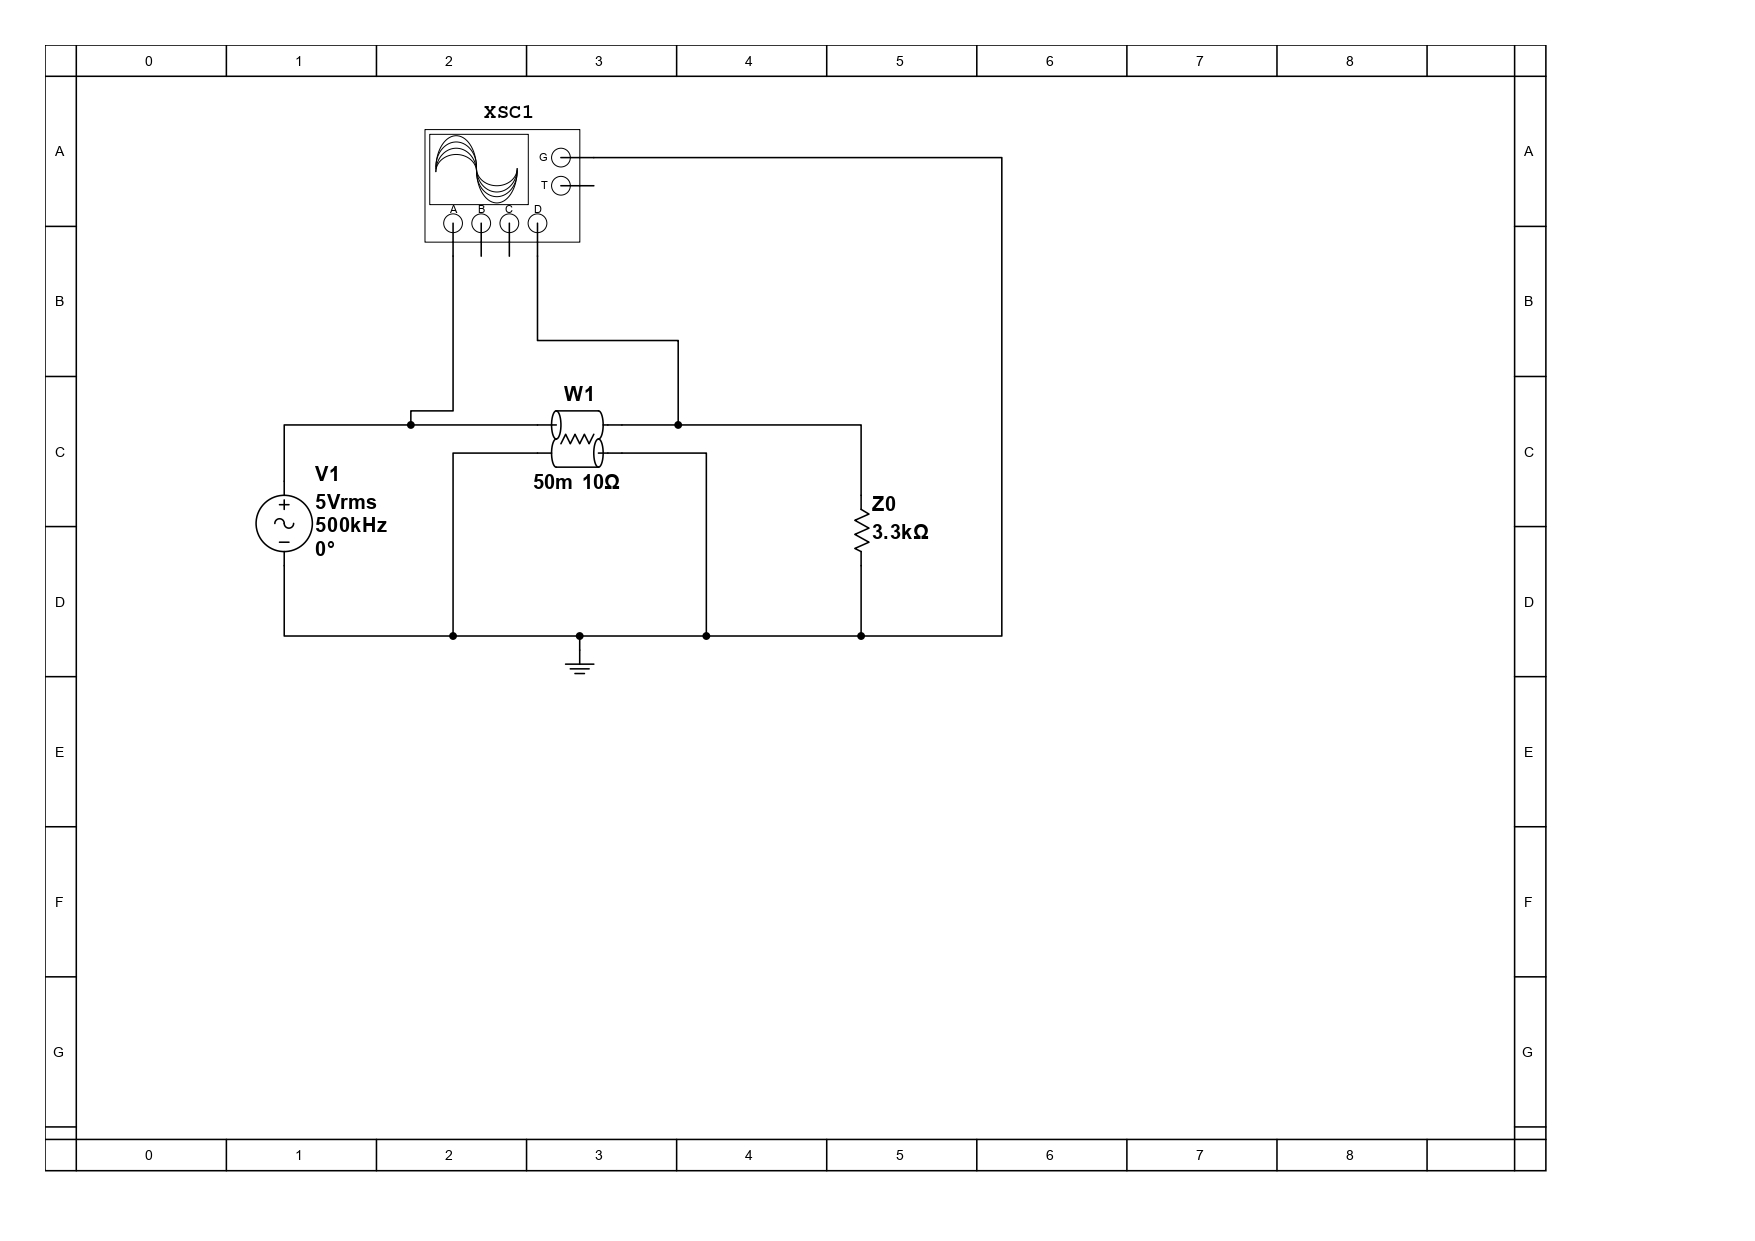
\includegraphics[width=1\linewidth]{1/scheme.jpg}
\subsection{<<ЛС с потерями в режиме несогласованной разомкнутой линии>>}
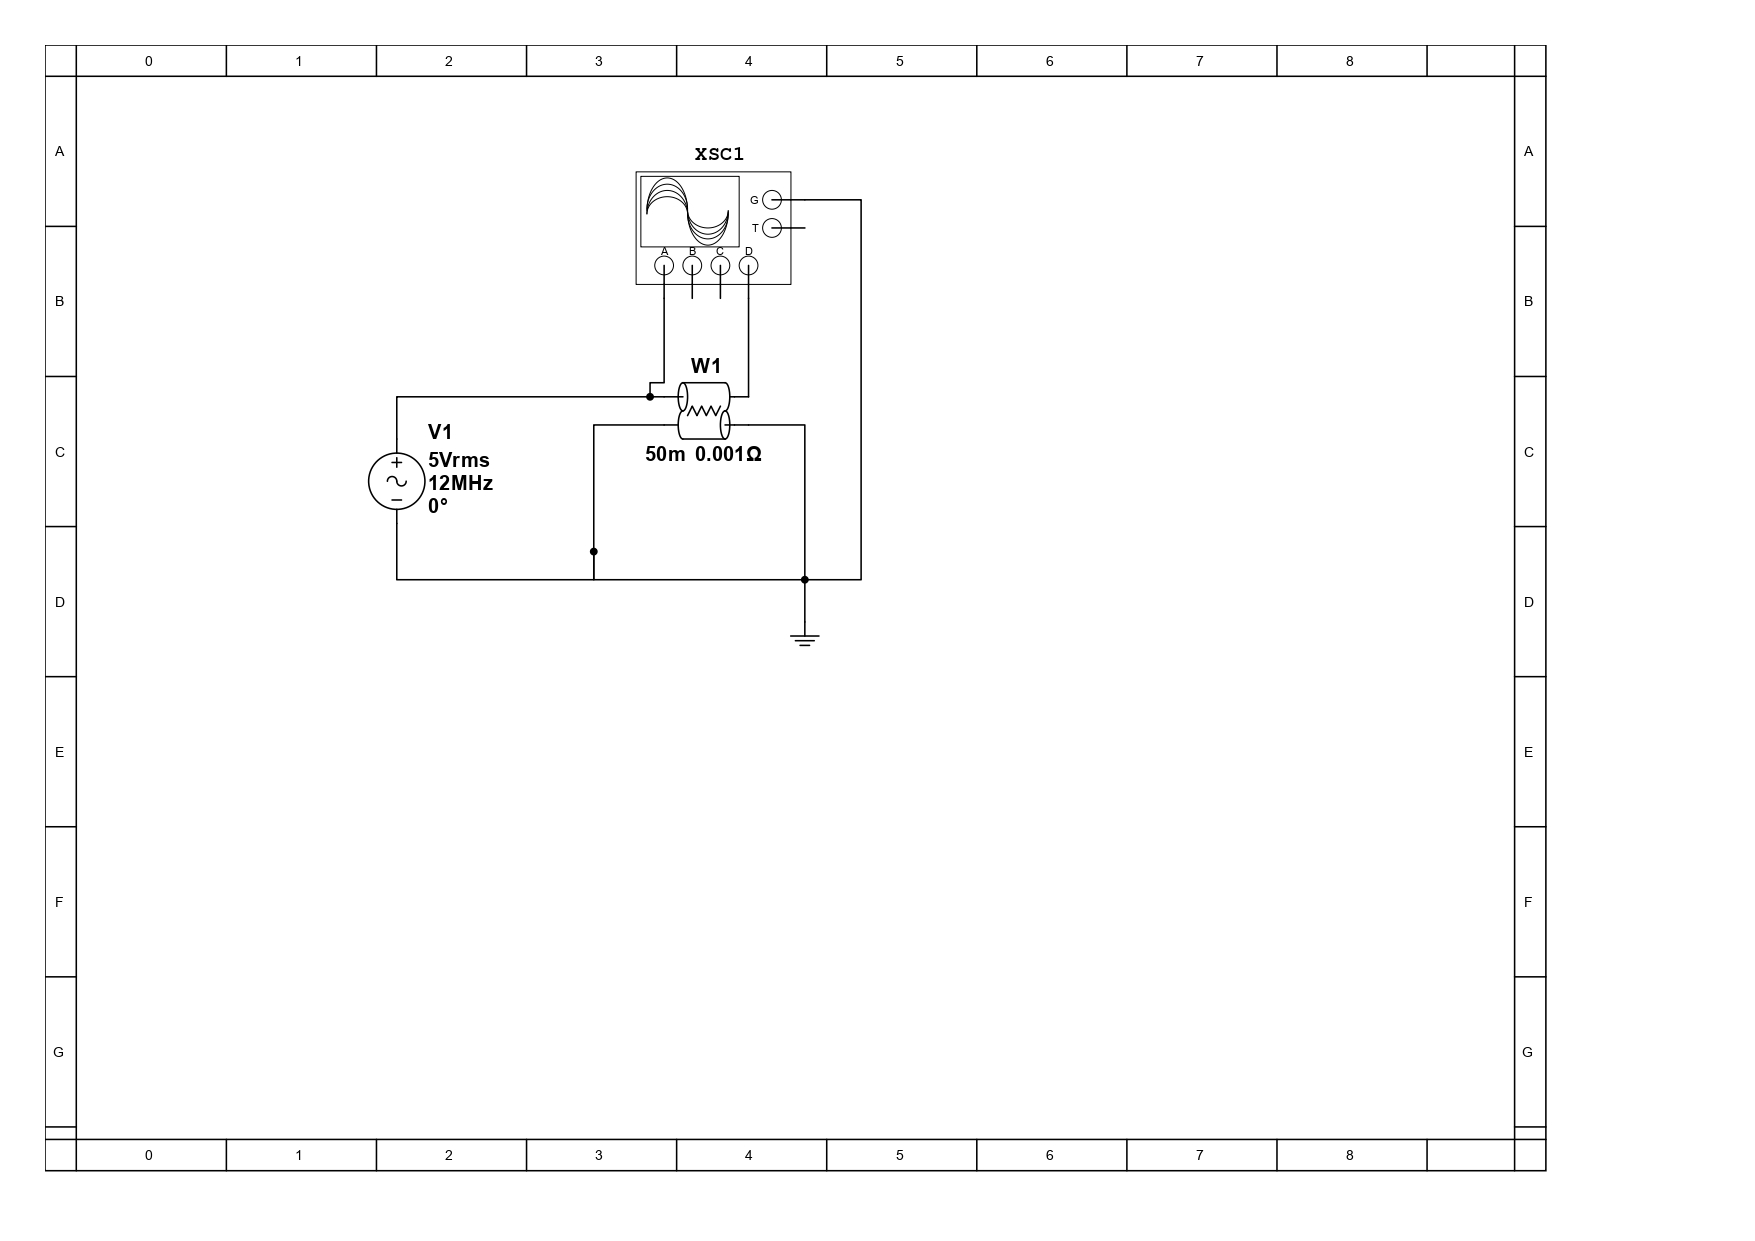
\includegraphics[width=1\linewidth]{2/scheme.jpg}
\subsection{<<ЛС с потерями в режиме несогласованной замкнутой линии>>}
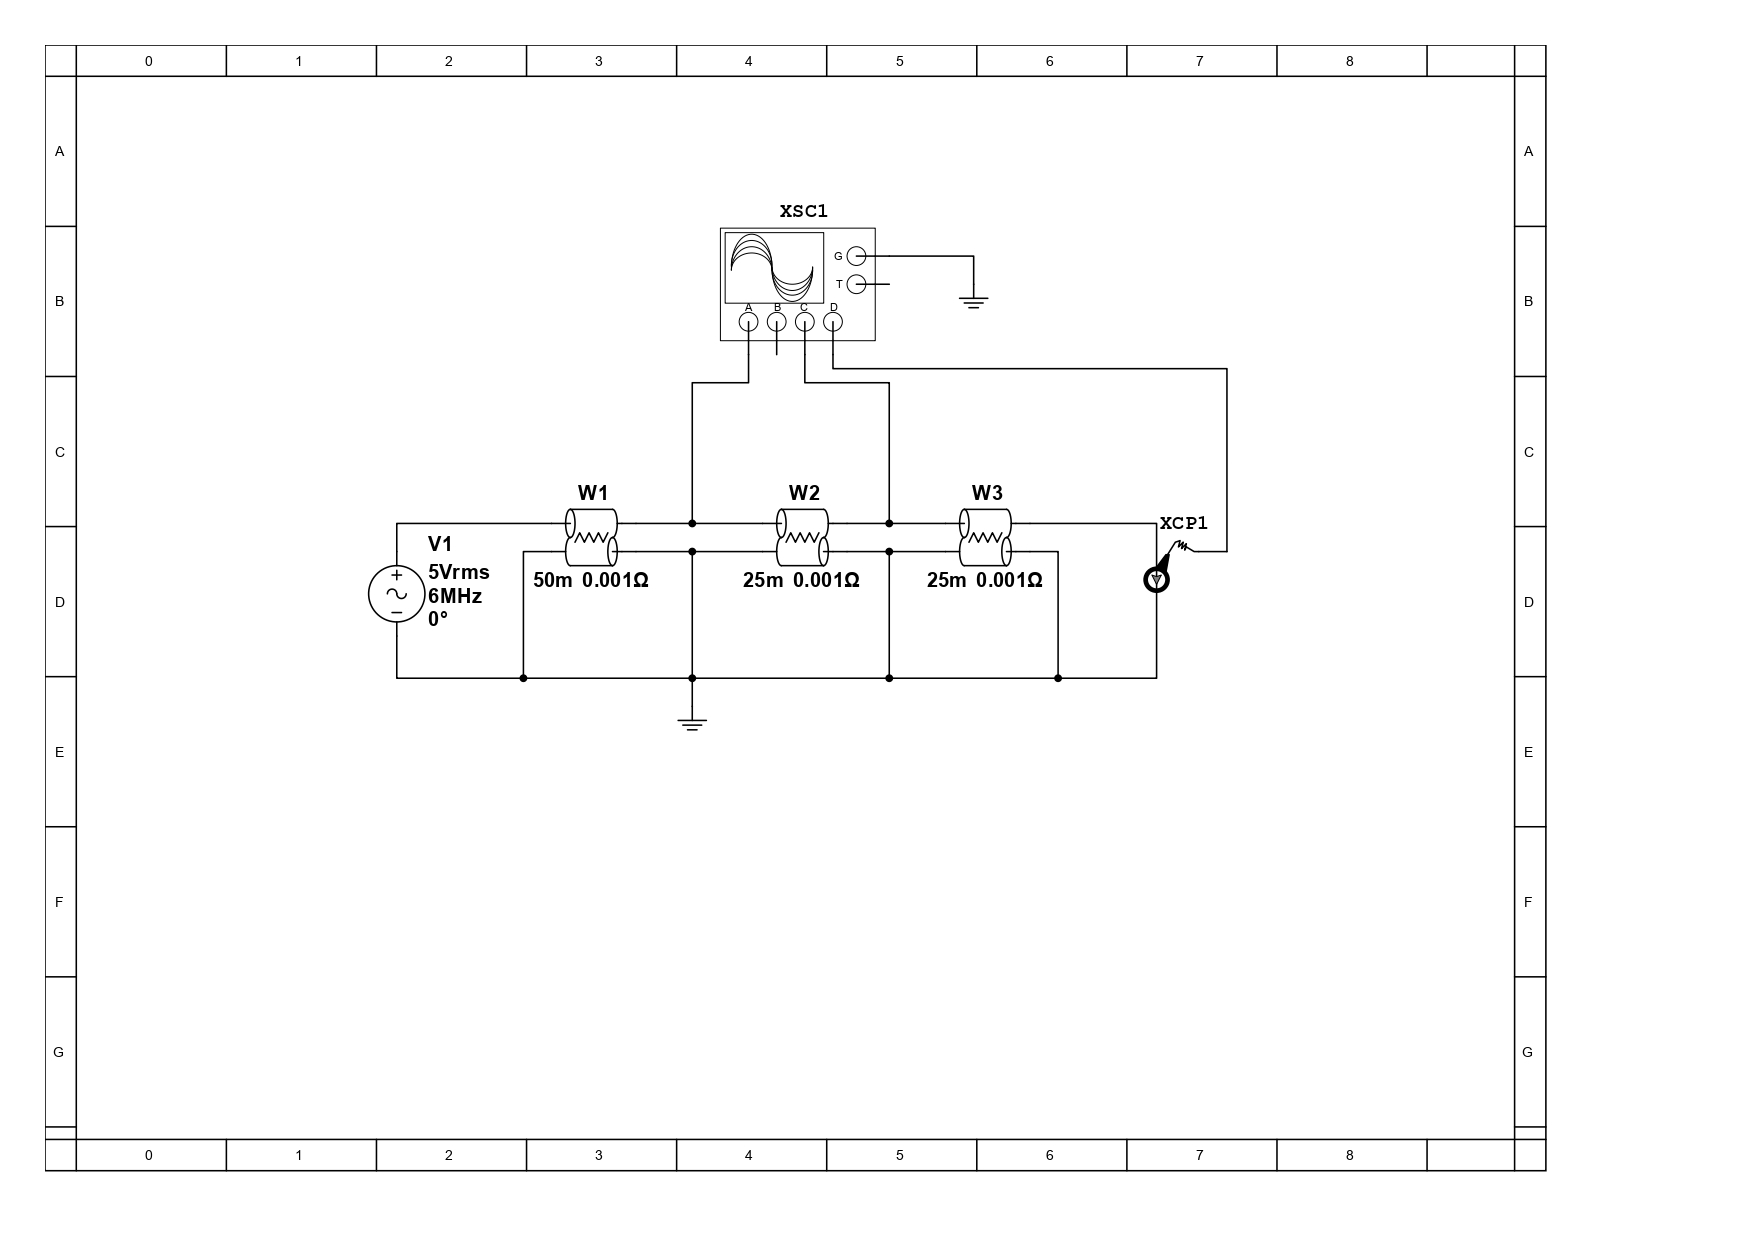
\includegraphics[width=1\linewidth]{3/scheme.jpg}
\subsection{<<ЛС с потерями в режиме несогласованной нагрузки>>}
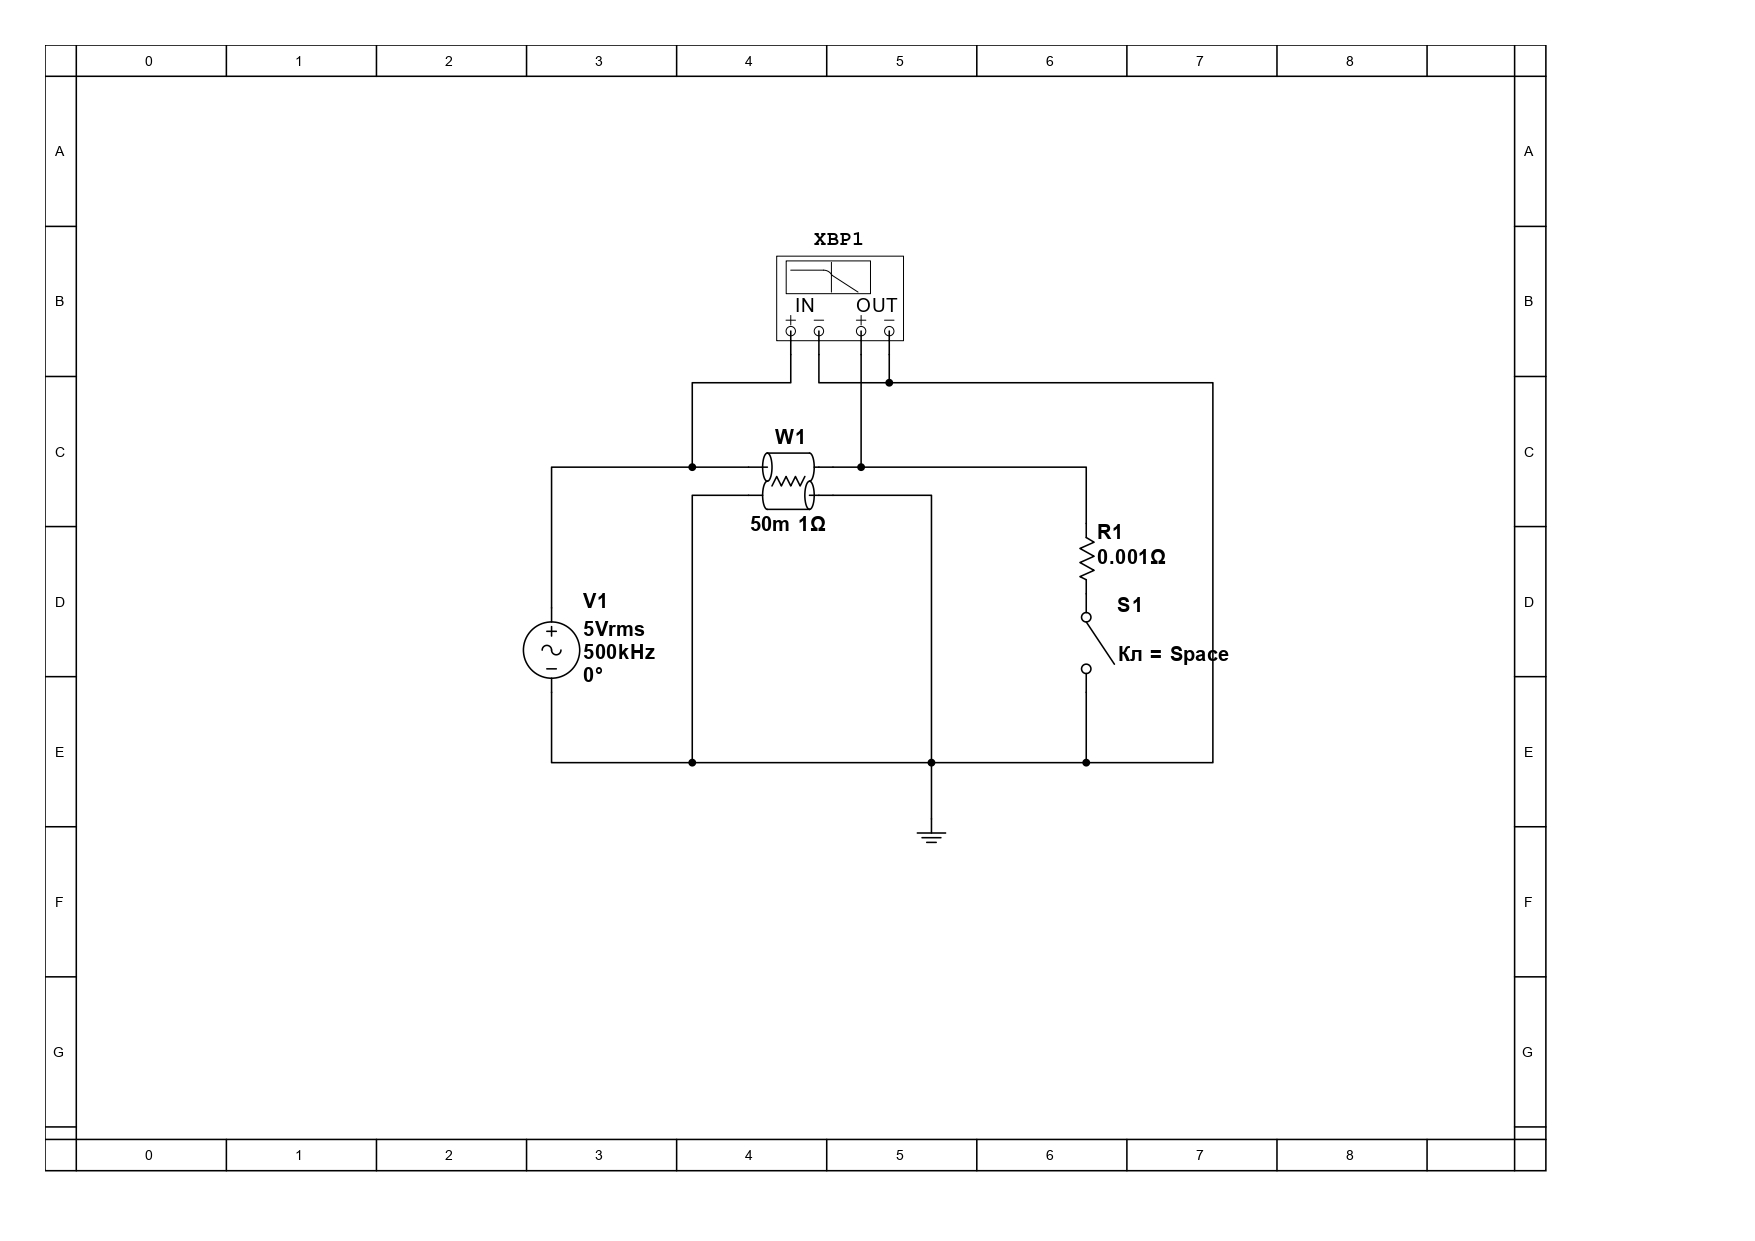
\includegraphics[width=1\linewidth]{4/scheme.jpg}
\section{Результаты расчетов и измерений приборами}
\subsection{<<ЛС в режиме согласованной линии>>}
Определим значения параметров $Z_0, C, G$:\\
$
Z_0 = \sqrt{\frac{L}{C}} = \sqrt{\frac{11,11\cdot 10^{-6}}{1\cdot 10^{-12}}}\approx 3,3\text{ кОм}\\
L*C = \frac{1}{c^2}=11,11\cdot 10^{-18}\Rightarrow C = \frac{11,11\cdot 10^{-18}}{11,11\cdot 10^{-6}} = 1 \text{ пФ}\\
G = \frac{RC}{L} = \frac{1\cdot 10^{-12}}{11,11\cdot 10^{-6}} = 9\cdot 10^{-8} = 90\cdot 10^{-9} = 90 \text{ нСм/м}\\
$
Исследуем модель линии связи для различных частот входного сигнала:
\begin{itemize}
    \item Осциллограмма при 500 кГц\\
        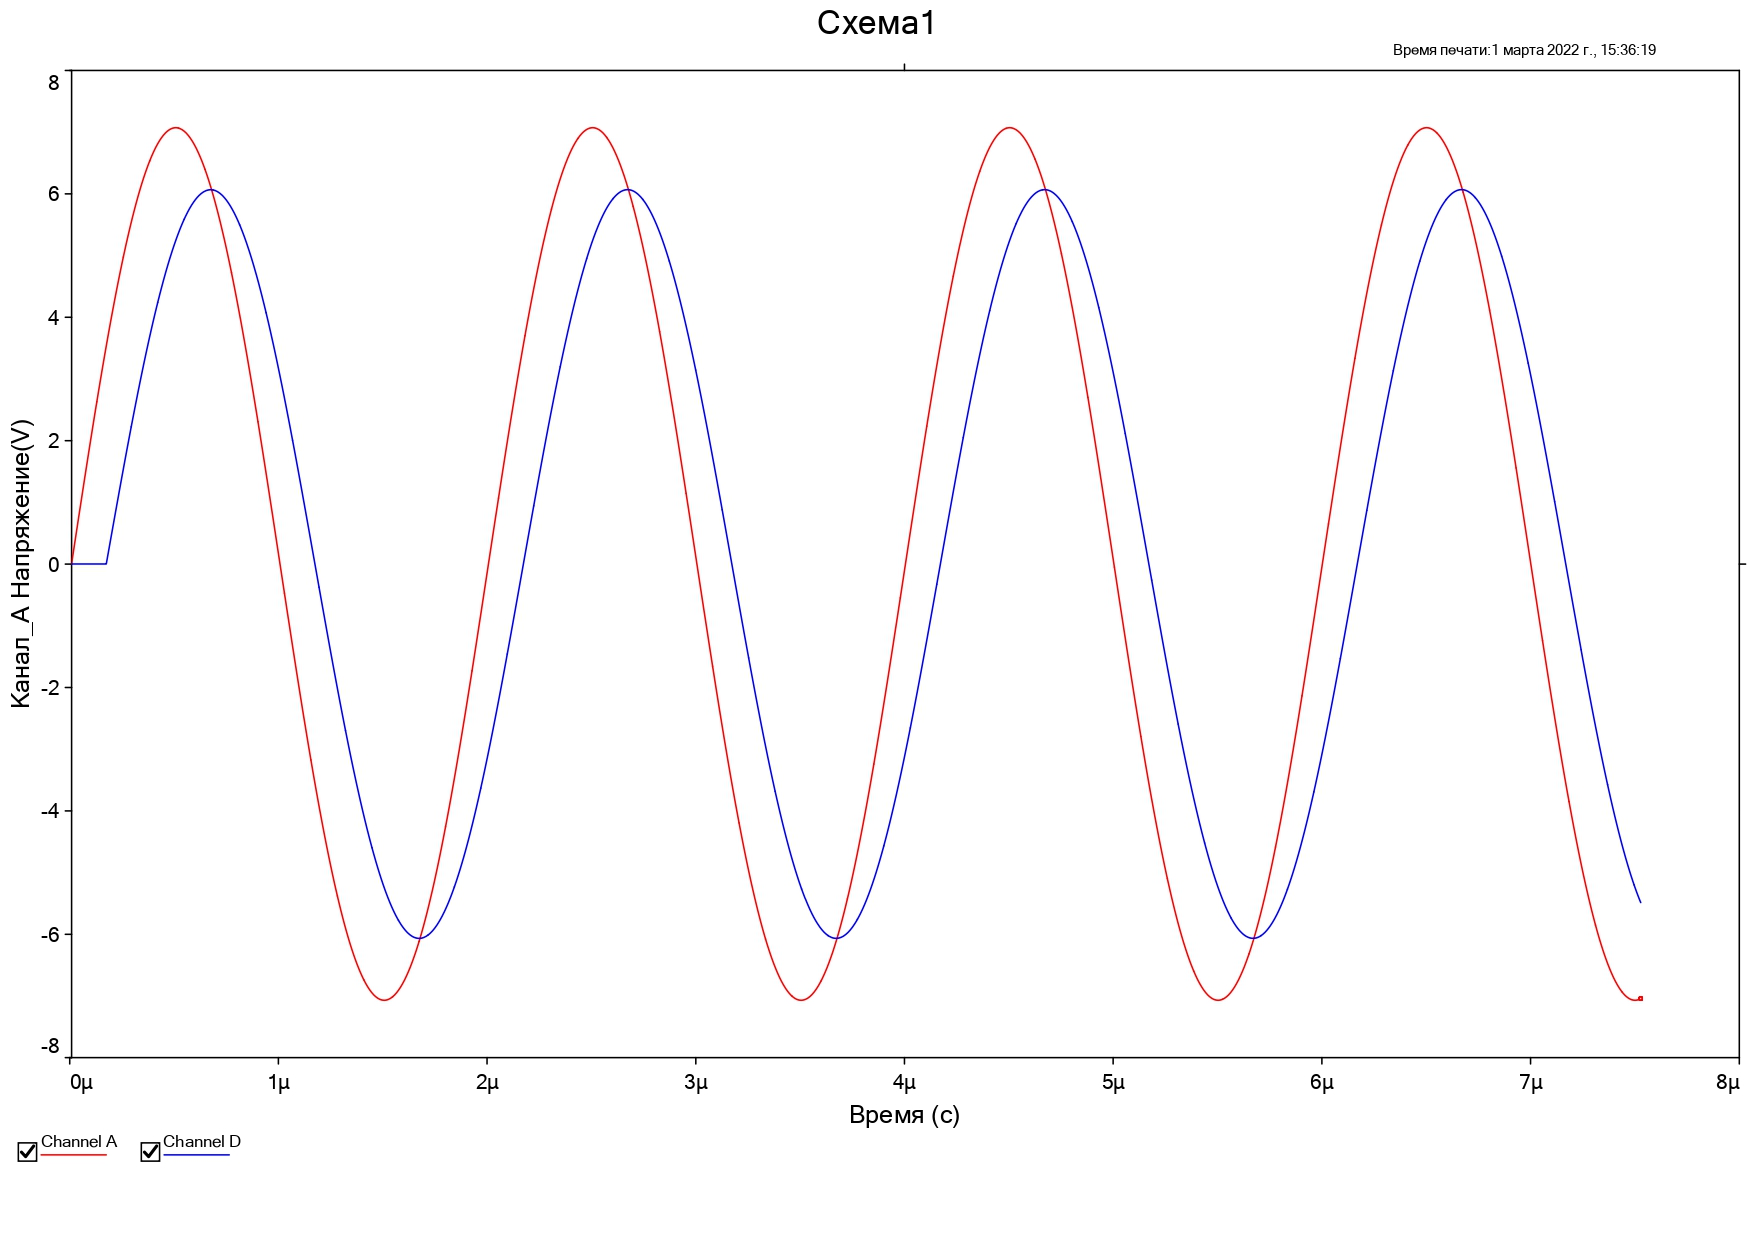
\includegraphics[width=1\linewidth]{1/500kgzosc.jpg}
    \item Осциллограмма при 800 кГц\\
        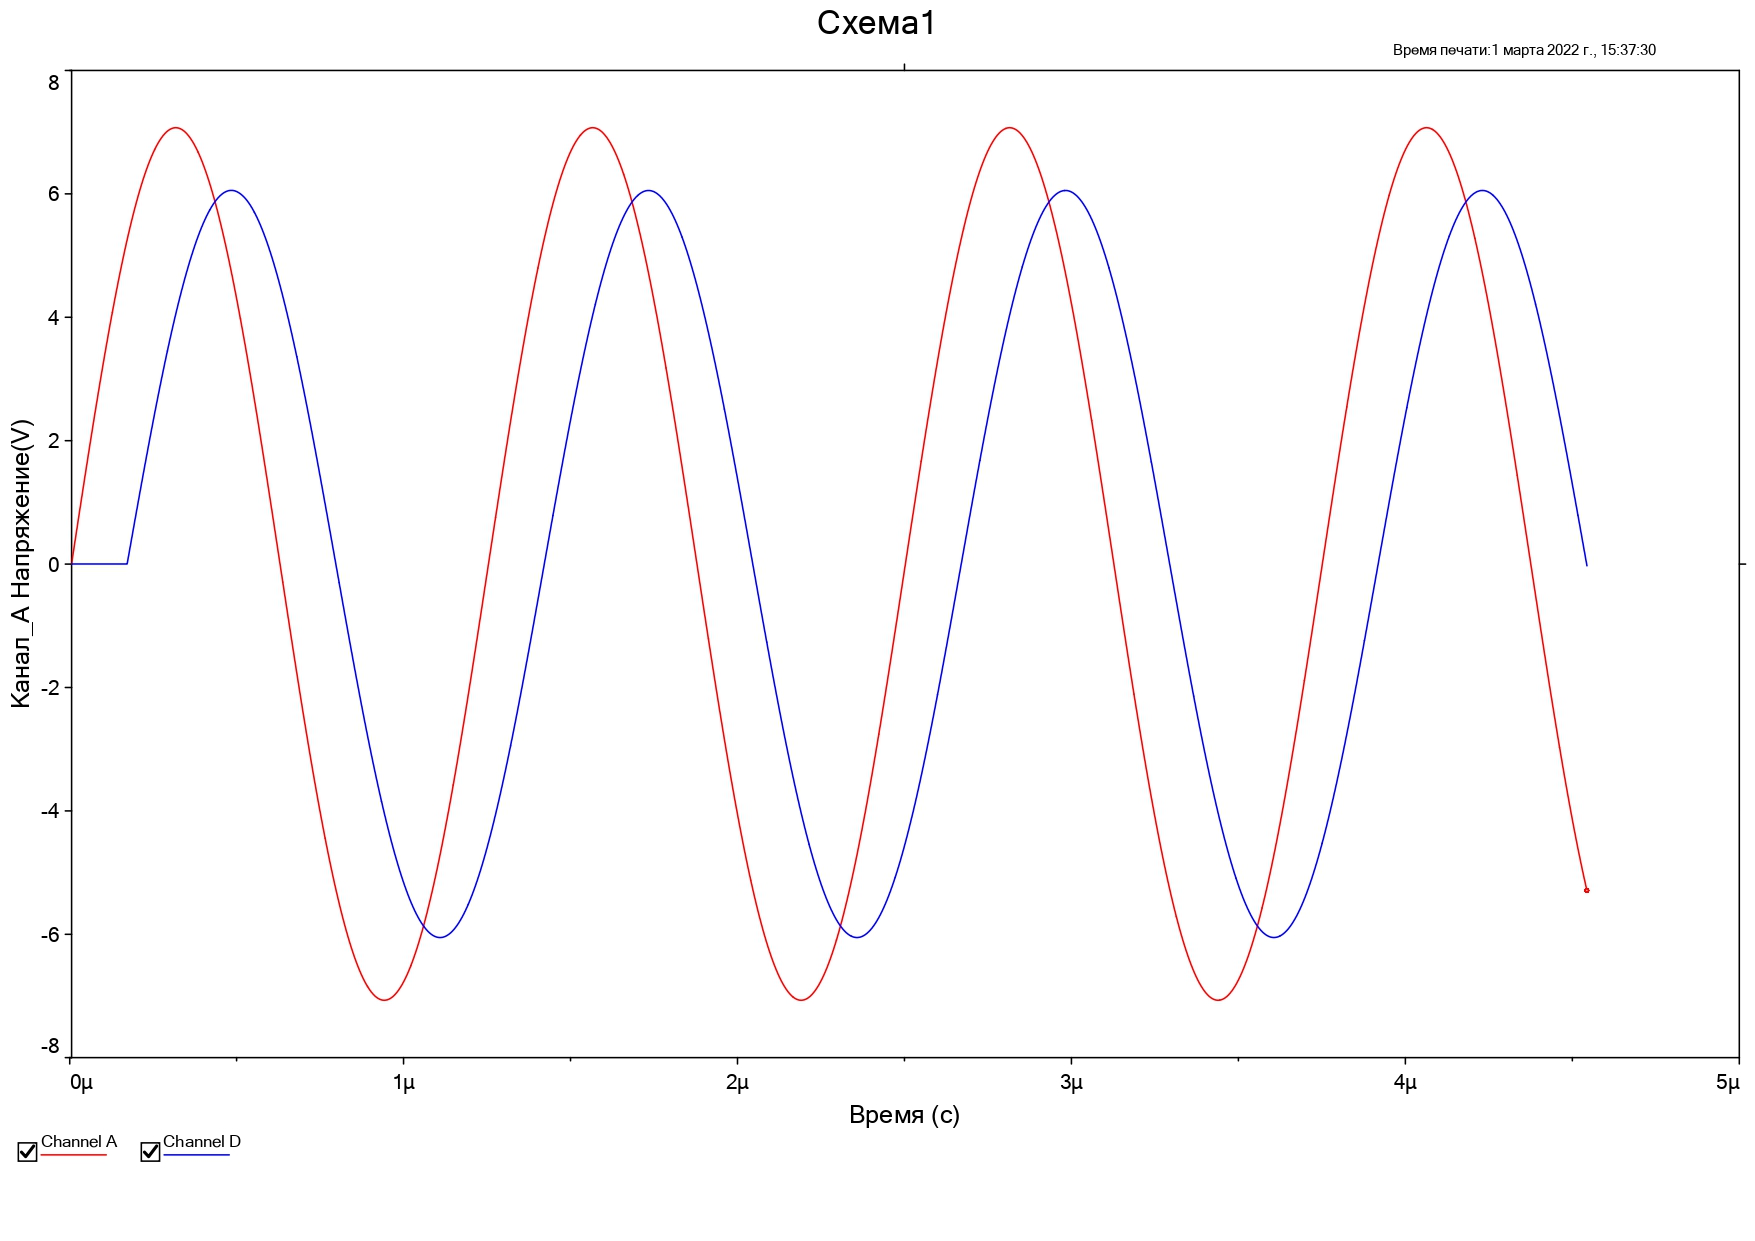
\includegraphics[width=1\linewidth]{1/800kgzosc.jpg}
\end{itemize}

\subsection{<<ЛС с потерями в режиме несогласованной разомкнутой линии>>}
\subsection{<<ЛС с потерями в режиме несогласованной замкнутой линии>>}
\subsection{<<ЛС с потерями в режиме несогласованной нагрузки>>}
\end{document}

